% Artyom Voronin
%  __  __           _      _ 
% |  \/  | ___   __| | ___| |
% | |\/| |/ _ \ / _` |/ _ \ |
% | |  | | (_) | (_| |  __/ |
% |_|  |_|\___/ \__,_|\___|_|
%                            
% Brno, 2020

% -------------------------------------------------------
% Section
% -------------------------------------------------------
\chapter{First Principle Modeling}
First-principle modeling is a common engineering modeling approach. Models
developed using physical laws such as energy and mass balance, heat
transfer, and so on. First-principle modeling requires knowledge of the
system and the physical processes that take place in this system.

First principle models (FPMs) are usually designed in the form of a system
of differential equations, algebraic differential equations, transfer
functions, state-space systems, etc.  In designing FPMs, it is necessary to
determine the assumptions and simplifications that correspond to the level
of technical resolution in a particular problem.

This chapter introduces the design of a double-acting pneumatic piston
assembly model, including sensors using a first-principle modeling
approach. 

% TODO Isermann Fault Detection str 72
%Measurements, Identification.

% Nonlinear dynamic modeling  Isermann FDS str. 84

% -------------------------------------------------------
%  __ _  ___ _ __   ___ _ __ __ _| |
% / _` |/ _ \ '_ \ / _ \ '__/ _` | |
%| (_| |  __/ | | |  __/ | | (_| | |
% \__, |\___|_| |_|\___|_|  \__,_|_|
% |___/                             
% -------------------------------------------------------
\section{General physical principles}
\paragraph{Assumptions}\label{assumptions}

\begin{enumerate}
    \item The effect of accelerated air mass is neglected. 
    \item The gas is ideal. 
    \item All the thermal processes are adiabatic.
\end{enumerate}


\paragraph{Equation of state}
Equation of state for an ideal gas \ref{eq:equation_of_state}, describe the relationships between
temperature, mass, pressure and volume of the gas, where $R=287.1 \rm [Jkg^{-1}K^{-1}]$ is an ideal gas
constant.

\begin{align}
    pV = mRT
    \label{eq:equation_of_state}
\end{align} 

\paragraph{Adiabatic process}
All processes take place without heat exchange with the environment by
given equation \ref{eq:adiabatic_process}, where $\kappa = c_p/c_v$ is a
heat capacity ratio.

\begin{align}
     p_1V_1^{\kappa} =  p_2V_2^{\kappa} = const
    \label{eq:adiabatic_process}
\end{align}

Relation between heat capacities and an ideal gas constant is given
by Mayer's equation as $c_p = c_v + R$.



\paragraph{Bernouilli's principle}
Bernouilli's equation \ref{eq:bernoullis_principle} describes flow
dynamics as a sum of kinetic, potential and internal energies.

\begin{align}
    H_1 + \frac{mw_1^2}{2} + mgz_1 + Q = H_2 + \frac{mw_2^2}{2} + mgz_w +
    W_T
    \label{eq:bernoullis_principle}
\end{align}

Transition to specific values:
\begin{align}
    h_1- h_2 = -\int_1^2 v dp = c_p(T_1-T_2) = 
    c_p T_1\left(1-\frac{T_2}{T_1}\right)
    \label{eq:etalpi_sub}
\end{align}

\paragraph{Continuity equation}
Continuity equation \ref{eq:continuity_equation} describes a mass flow
through a control volume.

\begin{align}
    \dot{m} = S_1 w_1 \rho_1 = S_2 w_2 \rho_2 = const
    \label{eq:continuity_equation}
\end{align}

\section{Air Expansion}
Air expansion from the reservoir, one of the fundamental sets of equations
used in pneumatic elements. 

\begin{figure}[h!]
    \centering
    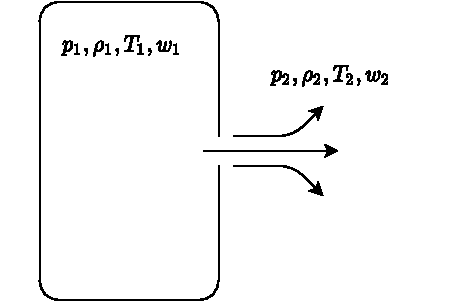
\includegraphics[width=0.5\textwidth]{air_tank.pdf}
    \caption{Air expansion from tank}
    \label{fig:air_expansion}
\end{figure}

Assuming that $W_T = 0, Q = 0$ there is no work and heat shared with the
the environment, there is no difference in height $z_1 = z_2$ and
the velocity difference is vast $w_2 << w_1$, applying equation
\ref{eq:bernoullis_principle}, get \ref{eq:w2}.


\begin{align}
    w_2 = \sqrt{2(h_1 - h_2)}
    \label{eq:w2}
\end{align}

\begin{align}
    w_2 = \sqrt{2c_p T_1 \left(1-\frac{T_2}{T_1}\right)}
    \label{eq:w2}
\end{align}

where 

\begin{align}
    T_1 = \frac{p_1}{R \rho_1} && 
    c_p = R  \left( \frac{\kappa}{\kappa-1} \right)   &&
    \frac{T_2}{T_1} = \left(\frac{p_2}{p_1} \right)^{\frac{\kappa - 1}{\kappa}}
    \label{eq:helpers}
\end{align}

Combine equations \ref{eq:w2}, \ref{eq:helpers} to get air expansion
velocity \ref{eq:w2_final}.

\begin{align}
    w_2 =
    \sqrt{2 \frac{\kappa}{\kappa-1} \frac{p_1}{\rho_1} 
    \left[(1-\left(\frac{p_2}{p_1}\right)^\frac{\kappa-1}{\kappa}\right]}
    \label{eq:w2_final}
\end{align}

From equations \ref{eq:helpers} express air density \ref{eq:rho2}.
\begin{align}
    \rho_2 = \frac{p_1}{RT_1} \left(\frac{p_2}{p_1}\right)^{\frac{1}{\kappa}}
    \label{eq:rho2}
\end{align}

Using continuity equation \ref{eq:continuity_equation} and
\ref{eq:w2_final} describe mass flow as \ref{eq:dot_m}:

\begin{align}
    \dot{m} = A p_1 \sqrt{\frac{2}{RT_1}}
    \sqrt{\frac{\kappa}{\kappa-1} \frac{p_1}{\rho_1} 
    \left[(1-\left(\frac{p_2}{p_1}\right)^\frac{\kappa-1}{\kappa}\right]}
    \label{eq:dot_m}
\end{align}

where \ref{eq:psi} is the outflow function.

\begin{align}
    \psi\left(\frac{p_2}{p_1}\right) =  
    \sqrt{\frac{\kappa}{\kappa-1} \frac{p_1}{\rho_1} 
    \left[(1-\left(\frac{p_2}{p_1}\right)^\frac{\kappa-1}{\kappa}\right]}
    \label{eq:psi}
\end{align}

Finally mass flow from the reservoir is given by equation \ref{eq:mass_flow}:
\begin{align}
    \dot{m} = A p_1\sqrt{\frac{2}{RT_1}} \cdot \psi\left(\frac{p_2}{p_1}\right)
    \label{eq:mass_flow}
\end{align}


\paragraph{Critical flow velocity}
The outflow function depends on the pressure ratio $p_2/p_1$. This function
has a maximum value when the critical pressure is reached; the mass flow
becomes chocked. Critical pressure is presented by \ref{eq:beta_k}. For the
overcritical pressure ratio, the mass flow depends only on $p_1$ and $T_1$
\cite{isermann}.

\begin{align}
    &\left(\frac{p_2}{p_1}\right)_{crit} =
    \left(\frac{2}{\kappa+1}\right)^\frac{\kappa}{\kappa-1}=\beta_k
    \label{eq:beta_k}
\end{align}

Critical pressure for air is $\beta_k = 0.528$ and critical velocity is
give by outflow function \ref{eq:psi_max}. Combine equations for
overcritical and undercritical pressure ratio using equations
\ref{eq:beta_k}, \ref{eq:psi_max} we get the final equation for overflow
function \ref{eq:psi_final}.

\begin{align}
    &\psi_{max} (\beta_k) = 
    \left(\frac{2}{\kappa+1}\right)^\frac{\kappa}{\kappa-1}\sqrt{\frac{\kappa}{\kappa+1}}
    = 0.484
    \label{eq:psi_max}
\end{align}

\begin{align}
\psi\left(\frac{p_2}{p_1}\right) = 
    \begin{cases}
    \sqrt{\frac{\kappa}{\kappa-1} \frac{p_1}{\rho_1} 
    \left[(1-\left(\frac{p_2}{p_1}\right)^\frac{\kappa-1}{\kappa}\right]}
    & 0.528 <\frac{p_2}{p_1} \le 1 \\
    \left(\frac{2}{\kappa +1}\right)^{\frac{1}{\kappa+1}}
    \sqrt{\frac{\kappa}{\kappa +1}} & 0 \le \frac{p2}{p1} \le 0.528\\
    \end{cases}
\label{eq:psi_final}
\end{align}

A detailed derivation of the equation \ref{eq:psi_final} can be found in
\cite{isermann},\cite{}.


%\begin{tabular}{ |c|c|c| }
%    \hline
%    $p$                     & $Pa$              & pressure \\
%    $V$                     & $m^3$             & volume \\
%    $m$                     & $kg$              & mass \\
%    $n$                     & $mol$             & amount of substance \\
%    $R$                     & $Jkg^{-1}K^{-1}$  & ideal gas constant \\
%    $r$                     & $Jkg^{-1}K^{-1}$  & mass-specific gas constant \\
%    $T$                     & $K$               & temperature \\
%    $S$                     & $m$               & area \\
%    $z$                     & $m$               & height \\
%    $w$                     & $ms^{-1}$         & flow speed \\
%    $H$                     & $J$               & enthalpy \\
%    $\nu$                   & $m^3kg^{-1}$      & specific volume \\
%    $Q$                     & $J$               & heat shared with
%                                                    environment \\
%    $W_T$                   & $J$               & work \\
%    $c_p$                   & $Jkg^{-1}K^{-1}$  & is the specific heat
%                                                    at constant pressure \\
%    $c_v$                   & $Jkg^{-1}K^{-1}$  & is the specific heat at constant volume\\
%    $g=9.81$                & $ms^{-2}$         & gravity acceleration \\
%    $\kappa=1.4\text{(air)}$& $-$               & heat capacity ratio
%                                                    (isentropic expansion factor)\\
%    \hline
%\end{tabular}


%\begin{tabular}{ |c|c|c| }
%    \hline
%    $\dot{m}$                   & $kgs^{-1}$  & mass flow \\
%    $c$                         & $ms^{-2}$   & speed of sound \\
%    $w_k$                       & $ms^{-2}$   & critical flow velocity \\
%    $\psi$                      & $-$         & flow coefficient \\
%    $\psi_{max}$                & $-$         & critical flow coefficient \\
%    $\beta$                     & $-$         & ration of pressure
%                                                    differential \\
%    $\beta_k$                   & $-$         & critical ratio of pressure
%                                                    differential \\
%
%    \hline
%\end{tabular}

% -------------------------------------------------------
% _ __  _ __ ___  ___ ___ _   _ _ __ ___ 
%| '_ \| '__/ _ \/ __/ __| | | | '__/ _ \
%| |_) | | |  __/\__ \__ \ |_| | | |  __/
%| .__/|_|  \___||___/___/\__,_|_|  \___|
%|_|                                     
% -------------------------------------------------------
\section{Pneumatic Piston Pressure Model}

%\begin{tabular}{ |c|c|c| }
%    \hline
%    $p_A, p_B$              & $Pa$              & pressure in chamber A, B \\
%    $\dot{m_A}, \dot{m_B}$  & $kg \cdot s^{-1}$ & mass flow on way to chamber A, B \\
%    $S_A, S_B$              & $m^2$             & piston area  \\
%    $V_A, V_B$              & $m^3$             & volume of chamber A,B \\
%    $V_{0A}, V_{0B}$        & $m^3$             & "dead" volume of chamber A,B \\
%    $m$                     & $kg$              & piston mass\\
%    $F_{load}$              & $N$               & load \\
%    $x$                     & $m$               & piston position \\
%    $l$                     & $m$               & maximum piston position \\
%    \hline
%\end{tabular}
A construction principle of the double-acting pneumatic piston is shown in
the figure \ref{fig:pist_chamb}.  There are two chambers connected to the control valve.
If the control valve is connected to chamber A, the supply pressure drives
mass flow into chamber A. At the same time, the port at chamber B is
connected to the ambient. Due to the pressure difference between chambers,
pneumatic piston stroke start moving in a positive direction. 
After the bound is reached and the pressure in the chamber equalizes to
supply pressure, there is no longer any mass flow coming inside.


\begin{figure}[h!]
    \centering
    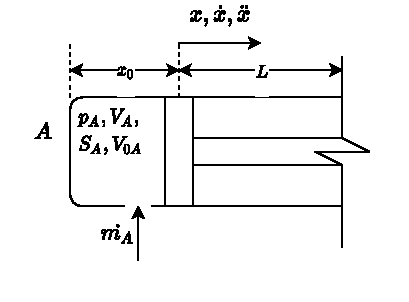
\includegraphics[width=0.6\textwidth]{pressure_chamber.pdf}
    \caption{Piston chamber}
    \label{fig:pist_chamb}
\end{figure}

Assuming an isothermal process, derivation of the equation of state $m =
\rho V$ get the equation \ref{eq:dm_state}. 

\begin{align}
    \dot{m} = \dot{\rho} V + \rho \dot{V}
    \label{eq:dm_state}
\end{align}

where

\begin{align}
    \rho = \frac{p}{RT} &&
    \dot{\rho} = \frac{\dot{p}}{RT} 
\end{align}

Equation \ref{eq:pressure1} describe pressure difference in chamber due
mass flow.
\begin{align}
    \dot{p} = - \frac{p}{V}\dot{V} + \frac{RT}{V}\dot{m}
    \label{eq:pressure1}
\end{align}


For the adiabatic model of the pressure difference in the chamber,
moreover, heat capacity ratio added
\ref{eq:pressure_adiabatic_simple_model}.

\begin{align}
    \dot{p} = - \frac{\kappa p}{V}\dot{V} + \frac{\kappa RT}{V}\dot{m}
    \label{eq:pressure_adiabatic_simple_model}
\end{align}
Volumes of the chambers can be represented concerning figure
\ref{fig:pist_chamb} as volumes equations \ref{eq:volumes}.

\begin{align}
    V_A = S_A x + V_{0A} \\
    V_B = S_B (L-x) + V_{0B} \\
    \dot{V}_A = S_A \dot{x} \\
    \dot{V}_B = - S_B \dot{x}
    \label{eq:volumes}
\end{align}

The pneumatic piston with chambers A, B is described by the system of
differential equations \ref{eq:p_A}, \ref{eq:p_B}. These equations describe a pneumatic
cylinder entirely. Furthermore, all the parameters can be directly measured
or found in the datasheet \cite{}.

\begin{align}
    \dot{p_A} = \frac{\kappa}{S_A x + V_{0A}} \left(- p_A S_A\dot{x} +
    RT_A\dot{m_A} \right)
    \label{eq:p_A}
\end{align}

\begin{align}
    \dot{p_B} = \frac{\kappa}{S_B (L-x) + V_{0B}} \left(p_B S_B\dot{x} +
    RT_B\dot{m_B} \right)
    \label{eq:p_B}
\end{align}


\section{Control Valve Model}

\subsection{Input/Output mass flows}

\begin{align}
    \dot{m}T = \dot{m_{in}}T_s - \dot{m_{out}}T_{A/B}
\end{align}



% TODO
\subsection{Valve model} 
\begin{tabular}{ |c|c|c| }
    \hline
    $S_{eq}$                & $m^2$         & Equivalent cross section \\
    $S_{max}$               & $m^2$         & Maximum cross section \\
    $Cd$                    & $-$           & Coefficient of contraction \\
    $u$                     & $-$           & Regulation variable \\
    \hline
\end{tabular}

\paragraph{Valve flow model with simply input control signal}
For regulation flow this model used input control signal directly without
spool mechanics.

Coefficient of contraction \ref{eq:coefficient_of_contraction}:
\begin{align}
    C_d = \frac{S_{eq}}{S_{max}}
    \label{eq:coefficient_of_contraction}
\end{align}

For flow control regulation $u \in \langle-1,1\rangle$ can be used.
\begin{align}
    u =
    \begin{cases}
        u \in \langle -1, 0) & \text{discharge the chamber} \\
        u = 0& \text{valve closed}  \\
        u \in (0, 1\rangle & \text{filling the chamber} 
    \end{cases}
\end{align} 

\begin{align}
    \dot{m} = u S_{max} C_d p_1 \sqrt{\frac{2}{RT_1}}
    \cdot \psi\left(\frac{p_2}{p_1}\right)
    \label{eq:flow}
\end{align}

\textbf{For filling the chamber:}
\begin{itemize}
\item $p_1 = p_s$ 
\item $p_2 = p_A \text{ or } p_B$
\item $T_1 = T_s$
\end{itemize}

\textbf{For discharge the chamber:}
\begin{itemize}
\item $p_1 = p_A \text{ or } p_B$
\item $p_2 = p_0$
\item $T_1 = T_A, T_B$
\end{itemize}

where $p_s$ is supply pressure. $p_0$ atmospheric pressure. As $T_i$ - 
atmospheric temperature using according to isothermal process.

\begin{align}
    \dot{m}_A =
    \begin{cases}
        u S_v C_d p_s \sqrt{\frac{2}{RT_s}}
        \cdot \psi\left(\frac{p_A}{p_s}\right)  &,   u \in (0, 1 \rangle \\
        0   &,  u = 0 \\
        u S_v C_d p_A \sqrt{\frac{2}{RT_A}}
        \cdot \psi\left(\frac{p_0}{p_A}\right)  &,   u \in \langle -1, 0) \\
    \end{cases}
\end{align}

\begin{align}
    \dot{m}_B =
    \begin{cases}
        u S_v C_d p_s \sqrt{\frac{2}{RT_s}}
        \cdot \psi\left(\frac{p_B}{p_s}\right)  &,   u \in (0, 1 \rangle \\
        0   &,  u = 0 \\
        u S_v C_d p_A \sqrt{\frac{2}{RT_B}}
        \cdot \psi\left(\frac{p_0}{p_B}\right)  &,   u \in \langle -1, 0) \\
    \end{cases}
\end{align}

\paragraph{Valve flow with spool mechanic included}

With respect to valve spool modeled as 1DOF system \ref{eq:1dof} and
mechanical and geometrical properties following equation were used.

\paragraph{Valve flow with spool}
In this model we accept a spool displacement $x_s$, controlled by input
voltage $u$.

\begin{equation}
    \dot{m}(P_u, P_d) = 
    \begin{cases}
        C_f A_v
        \left(\frac{\kappa}{R}\left(\frac{2}{\kappa-1}\right)\right)^{\frac{1}{2}}
        \cdot
        \frac{P_u}{\sqrt{T}}\left(\frac{P_d}{P_u}\right)^{\frac{1}{\kappa}}
        \cdot 
        \sqrt{1 - \left(\frac{P_d}{P_u}\right)^{\frac{\kappa-1}{\kappa}}} &,
            \text{ if } \frac{P_d}{P_u}>P_{cr} \text{ (subsonic)} \\
        C_f A_v \frac{P_u}{\sqrt{T}}\cdot \sqrt{\frac{\kappa}{R}
        \left(\frac{2}{\kappa + 1}\right)^{\frac{\kappa+1}{\kappa-1}}} &,
            \text{ if }  \frac{P_d}{P_u} \le P_{cr} \text{ (sonic)} \\
    \end{cases}
    \label{eq:valve_2}
\end{equation}

where $C_f$ is discharge coefficient, $A_v$ is the effective are of valve
orifice.

\begin{equation}
    A_v = \frac{\pi x_s^2}{4}
    \label{eq:A_v}
\end{equation}

\begin{equation}
    x_s = C_v u
    \label{eq:x_s}
\end{equation}

where $C_v$ is the valve constant.

\paragraph{Valve model by Endler}
Require fitting constants and generally system identification.
Mass flow rates are given by following equations:


\begin{equation}
    \begin{aligned}
        \dot{m}_A(u, p_A) = g_1(p_A, sign(u))arctg(2u) \\
        \dot{m}_B(u, p_B) = g_2(p_B, sign(u))arctg(2u)
    \end{aligned}
\end{equation}

where $g_1, g_2$ are signal functions given:
\begin{equation}
    \begin{aligned}
        g_1(p_A, sign(u)) = \beta \Delta p_A = 
        \begin{cases}
            (p_s - p_A) \beta^{ench} &, \rm \ if\  u \ge 0 \\
            (p_A - p_0) \beta^{esv} &, \rm \ if\  u  < 0 \\
        \end{cases} \\
        g_2(p_B, sign(u)) = \beta \Delta p_B = 
        \begin{cases}
            (p_s - p_B) \beta^{ench} &, \rm \ if\  u < 0 \\
            (p_B - p_0) \beta^{esv} &, \rm \ if\  u \ge 0 \\
        \end{cases}
    \end{aligned}
    \label{eq:valve_3}
\end{equation}

where $\beta^{ench}, \beta^{evs}$ are constant coefficients.
For fitting model stop piston (speed of piston is null). This mean that
volume is constant. We can measure flow rate $\dot{m}$ versus input voltage
$u$ with given pressure difference.

\paragraph{Valve dead-zone}
For more precision control and modeling of the valve system, valve
dead-zone can be used \ref{eq:deadzone}.

\begin{equation}
    u_z = 
    \begin{cases}
        g_z(u) < 0 &, \text{ if } u \le u_n \\
        0          &, \text{ if } u_n < u < u_p \\
        h_z(u) > 0 &, \text{ if } u \ge u_p \\
    \end{cases}  
    \label{eq:deadzone}
\end{equation}



% -------------------------------------------------------
% _ __ ___   ___  ___| |__   __ _ _ __ (_) ___ 
%| '_ ` _ \ / _ \/ __| '_ \ / _` | '_ \| |/ __|
%| | | | | |  __/ (__| | | | (_| | | | | | (__ 
%|_| |_| |_|\___|\___|_| |_|\__,_|_| |_|_|\___|
% -------------------------------------------------------
\section{Mechanical assembly}
\subsection{Equation of motion}

The motion of the pneumatic piston mechanism describes in terms of the
general 1dof dynamical equation \ref{eq:1dof}. 

\begin{equation}
    m\ddot{x} + b\dot{x} + kx = u
    \label{eq:1dof}
\end{equation}

In the case of the pneumatic piston, the equation \ref{eq:1dof}
transforms into an equation \ref{eq:mechanical}.

\begin{equation}
    (M + M_L) \ddot{x} + F_{damp} + F_g + F_{hs}  = F_p
    \label{eq:mechanical}
\end{equation}

Where $M$ represents a mass of the all moveable part of the piston,
$M_L$ is load mass, $F_g$ gravity force acting to mechanical moving assembly,
$F_{hs}$ - models endpoints (hard stop),
$F_{damp}$ represents shock absorbers acted at endpoints,
$F_{p}$ is a force produced by the pneumatic piston \ref{eq:pneum}.

\begin{equation}
    F_p = P_A S_A - P_B S_B - P_0 S_0
    \label{eq:pneum}
\end{equation}

\subsection{Hard stop}
Hard stop can be represented as spring and dumps:

\begin{align}
    F_{HS} =
    \begin{cases}
        K_p(x-g_p) + D_pv & \text{for } x \ge g_p \\
        0 & \text{for } g_n < x < g_p \\
        K_n(x-g_n) + D_nv & \text{for } x \le g_n \\
    \end{cases}
\end{align}


\subsection{Shock Absorbers}
\subsection{Friction}
Friction force can be modeled in the
different ways.

TO MUCH
\ref{eq:friction1}.
\begin{equation}
    F_f = 
    \begin{cases}
        C \dot{x} + \left(f_c + (f_s-f_c)
        e^{-\left(\frac{\dot{x}}{v_s}\right)^{\delta}}\right) sign(\dot{x}) &,
        \text{ if } \dot{x} \le v_e \\
        \mu \dot{x} &,
        \text{ if } \dot{x} > v_e \\
    \end{cases}
    \label{eq:friction1}
\end{equation}
where $C$ - viscous friction coefficient, $f_c$ - Coulomb friction, $f_s$ -
maximum static friction, $\mu$ - dynamic friction factor, $v_s$ - Stribeck velocity,
$\delta$ - arbitrary index, $v_e$ critical velocity.


% -------------------------------------------------------
% ___  ___ _ __  ___  ___  _ __ ___ 
%/ __|/ _ \ '_ \/ __|/ _ \| '__/ __|
%\__ \  __/ | | \__ \ (_) | |  \__ \
%|___/\___|_| |_|___/\___/|_|  |___/
% -------------------------------------------------------
\section{Sensors Modeling}
\begin{itemize}
    \item Sensors models
\end{itemize}

% -------------------------------------------------------
%(_) __| | ___ _ __ | |_ 
%| |/ _` |/ _ \ '_ \| __|
%| | (_| |  __/ | | | |_ 
%|_|\__,_|\___|_| |_|\__|
% -------------------------------------------------------
\section{Parameter identification}

\subsection{Mechanical assembly}
In mechanical system there is $F_f$ force represented by frictions accruing
in the system. This force can be modeled by different friction models with
respect to \ref{sec:mech_assembly}. Friction force parameters can be
estimated using "gray-box" method. 
Using $\dot{m}$ mass flow data versus $x$ position measured on real assembly
and use these data as an input and output, we can fit $F_f$.
Simplify model can contain TODO:
\begin{itemize}
    \item $F_C$ static friction
    \item $C_v$ viscous
    \item $C_p$ Pressure difference
\end{itemize}

\subsection{Cylinder}
Dead volume: $p_1 V_1^n = p_2 V_2^n$ or datasheet.

\subsection{Valve}
For valve system there are two parameters that need to be estimated.
According to equation \ref{eq:flow2} with constant $p_1$ (pressure supply) and $p_2$
(atmospheric pressure), we can estimate $\boldsymbol{C}$ if we neglect Valve Spool dynamic.
If in experiment we determine that spool dynamic necessary to include. We
provide same experiment with spool model including to "Gray-box" fitting
model.
\begin{align}
    \dot{m} = \boldsymbol{u}(x_s) \boldsymbol{C}  p_1 \sqrt{\frac{2}{RT_1}}
    \cdot \psi\left(\frac{p_2}{p_1}\right)
    \label{eq:flow2}
\end{align}



